% \vspace{-6mm}
\section*{A Guide: Resources for Best Development Practices}
\label{sec:guide}

\paragraph{Why?} 
This cheatsheet serves as a succinct guide, prepared \emph{by} foundation model developers \emph{for} foundation model developers.
The intended audience is a range of foundation model developers, including academic researchers, startup companies, research labs, who are pretraining from scratch, or simply finetuning, big and small.
As the field of AI foundation model development rapidly expands, welcoming new contributors, scientists, and applications, we hope to lower the barrier for new community members to become familiar with the variety of resources, tools, and findings.
The focus of this cheatsheet is not only, or even primarily, to support building, but to inculcate good practices, awareness of limitations, and general responsible habits as community norms.
While it is certainly not comprehensive, we have selected a sample of resources that we have found useful and would recommend for consideration by others.
We hope it will serve as a general guide to promote responsible development practices, as well as building new models and infrastructure in our field.
%This document provides contextualized information and a static sample of the cheatsheet---the fully documented, live cheatsheet is available at \url{fmcheatsheet.org}.

% \vspace{-2mm}
\paragraph{What?}
There are many exceedingly popular tools to build, distribute and deploy foundation models.
But there are also many outstanding resources that receive less attention or adoption, in part because of developers' haste to accelerate, deploy, and monetize.
We hope to bring wider attention to these core resources that support \emph{informed} data selection, processing, and understanding (\cref{sec:data,sec:data-prep}), \emph{precise and limitation-aware} artifact documentation (\cref{sec:documentation}), \emph{efficient} model training (\cref{sec:model-training}), \emph{advance awareness} of the environmental impact from training (\cref{sec:environmental-impact}), \emph{careful} model evaluation of capabilities, risks, and claims (\cref{sec:model-eval}), as well as \emph{responsible} model release and deployment practices (\cref{sec:model-release}).

In each section we introduce considerations for that phase of development.
We suggest developers building models from scratch carefully consider their data sources and curation processes to avoid unintended risk (e.g. privacy, copyright, inappropriate content), marginalization (e.g. by accidental filtering), or unexpected model behaviors (e.g. text distribution has unintended quirks). 
Data processing should consider how to deduplicate, filter, decontaminate, and mix different data sources towards the intended distribution and characteristics.
We recommend this process is carefully documented for reproducibility and understanding.
If new data is released, setting its governance standards early will avoid misuse later, and adding structure to documentation will allow for its properties to be easily preserved, understood, and respected in downstream data mixes or compositions.
Model training can be financially and environmentally expensive.
Resources for estimating environmental impact can break down these costs and simplify the considerations.
Newly trained models should be carefully evaluated for their intended uses, as well as foreseeable misuses or harms.
We suggest resources to taxonomize and contextualize evaluations, without over-claiming or misunderstanding the limitations of the reported numbers.
Lastly, we suggest how developers can make an informed selection of licenses, and release mechanisms, to mitigate potential misuses.


% \vspace{-2mm}
\paragraph{Criteria for Inclusion.}
\label{sec:criteria}
The resources are selected based on a literature review for each phase of foundation model development. Inclusion is predicated on a series of considerations, including: the perceived helpfulness as a development tool, the extent and quality of the documentation, the insights brought to the development process, and, in some cases, the lack of awareness a useful resource has received in the AI community.
For an example of this last consideration, in \cref{sec:finetune} we try to include more Finetuning Data Catalogs for lower resource languages, that often receive less attention than HuggingFace's Dataset library.
Rather than sharing primarily academic literature as in a traditional survey work, we focus on tools, such as data catalogs, search/analysis tools, evaluation repositories, and, selectively, literature that summarizes, surveys or guides important development decisions.
As with any survey, these principles for inclusion are incomplete and subjective, but we hope to remedy this with the open call for community contributions.

% \vspace{-2mm}
\paragraph{How to contribute?}
We intend for the web version of the cheatsheet to be a crowdsourced, interactive, living document, with search and filter tools.
To contribute to this resource, follow instructions given in the website.
Contributions should be scoped to resources, such as tools, artifacts, or helpful context papers, that directly inform responsible foundation model development.
Significant contributions will be recognized in the web search tool, and in follow up write-ups to this guide.
Contributed content will be reviewed by authors, to assess that the resources fit the aspirational criteria for inclusion outlined above.

% \vspace{-2mm}
\paragraph{Scope \& Limitations.} 
We've compiled resources, tools, and papers that have helped guide our own intuitions around model development, and which we believe will be especially helpful to nascent (and sometimes even experienced) developers in the field.
However, this guide is far from exhaustive---and here's what to consider when using it:

\begin{itemize} %[itemsep=1pt]%, wide=5pt]
    \item We scope these resources to newer foundation model developers, usually releasing models to the community. Larger organizations, with commercial services, have even broader considerations for responsible development and release.
    \item Foundation model development is a rapidly evolving science. %\textbf{This document is only a sample, dated to January 2024.} The full cheatsheet is more comprehensive and open for on-going public contributions: \url{fmcheatsheet.org}.
    \item We've scoped our data modalities only to \textbf{text, vision, and speech}. 
    We support multilingual resources, but acknowledge this is only a starting point.
    \item A cheatsheet \textbf{cannot be comprehensive}. We prioritize resources we have found helpful, and rely heavily on survey papers and repositories to point out the many other awesome works which deserve consideration, especially for developers who plan to dive deeper into a topic.
    \item \textbf{We cannot take responsibility for these resources---onus is on the reader to assess their viability, particularly for their circumstance.} At times we have provided resources with conflicting advice, as it is helpful to be aware of divided community perspectives. Our notes throughout are designed to contextualize these resources, to help guide the reader's judgement.
\end{itemize}

% \vspace{-2mm}
\paragraph{Notations and Symbols}
This cheatsheet provides tables for several topics, with symbols for brevity.
Modalities are indicated for text ~\TextCircle[0.75]{}, vision~\VisionCircle[0.75]{}, and speech ~\SpeechCircle[0.75].
We also provide hyperlinks for ArXiv \earxiv[1.2em][-0.4ex]\hspace{0.25em}, for Hugging Face objects \ehf[1.2em][-0.4ex]\hspace{0.25em}, for GitHub \egithub[1.2em][-0.4ex]\hspace{0.25em}, and for webpages \eweb[1.2em][-0.4ex]\hspace{0.25em}.

% \vspace{-2mm}
\paragraph{Who are we?}
An organic collective of volunteers have contributed to this cheatsheet, spanning developers of several notable datasets (MasakhaNER \citep{adelani2021masakhaner}, the Pile \citep{gao2020pile}, ROOTS \citep{NEURIPS2022_ce9e92e3}, Dolma \citep{dolma}, the Flan Collection \citep{longpre2023flan}, the Data Provenance Collection \citep{longpre2023data}), models (OpenFlamingo \citep{awadalla2023openflamingo}, Pythia \citep{biderman2023pythia}, Flan-PaLM \citep{chung2022scaling}, RWKV \citep{peng2023rwkv}), and benchmarks (LM Eval Harness \citep{eval-harness}, HELM \citep{liang2022holistic}) in the community.
Most importantly, contributors (\cref{app:contributions}) have carefully assembled the tools and resources that have enabled them to build this infrastructure responsibly with an eye on social and scientific impact.

\begin{figure*}[ht]
    \centering
    \begin{subfigure}{0.94\textwidth}
        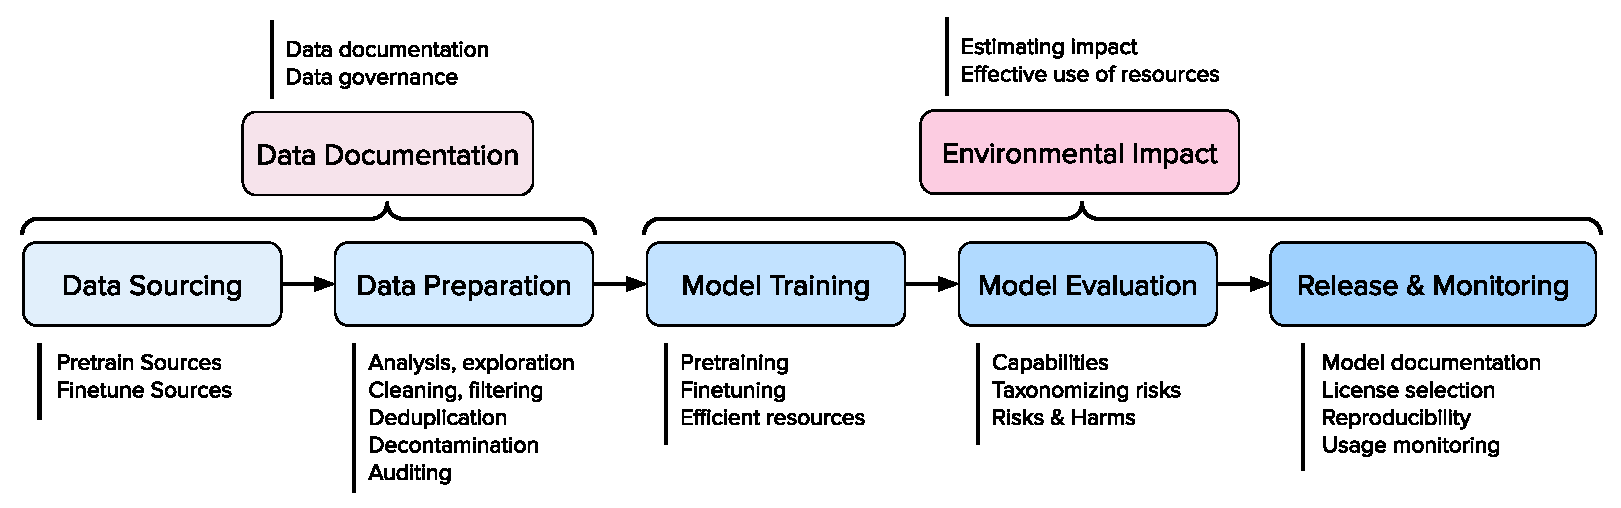
\includegraphics[width=\textwidth]{logos/cheatsheet-flow.pdf}
    \end{subfigure}
    % \caption{\textbf{} }
    \label{fig:cheatsheet-flow}
    \vspace{-3mm}
\end{figure*}

% \begin{table*}[t!]
% \centering
% \footnotesize
% % \renewcommand{\arraystretch}{1.5}
% \begin{adjustbox}{width=\textwidth}
% \begin{tabular}{p{3cm} p{13cm}}
% \toprule
% \textbf{Section} & \textbf{Review Summary}\\
% \midrule

% \multirow{4}{*}{Data Sources} & The community would benefit from more accurate and comprehensive licensing, provenance, and creator consent information for existing datasets. \\
% & \cellcolor[gray]{0.9}The community would benefit from more accurate and comprehensive information on sensitive content, such
% as CSAM and NCII. \\
% & Data \& modeling have focused predominantly on easy-to-scale data formats, neglecting other formats. \\
% & \cellcolor[gray]{0.9}There is a scarcity of realistic training tasks, and naturalistic observations. \\
% \midrule
% \multirow{6}{*}{Data Preparation} & Placeholder. \\
% & \cellcolor[gray]{0.9}Placeholder. \\
% & Placeholder. \\
% & \cellcolor[gray]{0.9}Placeholder. \\
% & Placeholder. \\
% & \cellcolor[gray]{0.9}Placeholder. \\
% \midrule
% \multirow{3}{*}{Data Documentation \& Release} & Placeholder. \\
% & \cellcolor[gray]{0.9}Placeholder. \\
% & Placeholder. \\
% \midrule
% \multirow{4}{*}{Model Training} & Placeholder. \\
% & \cellcolor[gray]{0.9}Placeholder. \\
% & Placeholder. \\
% & \cellcolor[gray]{0.9}Placeholder. \\
% \midrule
% \multirow{5}{*}{Environmental Impact} & Transparency from consumer-level API providers, into query-level energy and environmental usage measures. \\
% & \cellcolor[gray]{0.9}Transparency from hardware makers and data centers, into fine-grained energy and environmental usage measures. \\
% & ``Energy Star'' standards for non-technical users to fairly compare AI services. \\
% & \cellcolor[gray]{0.9}Scaling laws research currently lacks empirical evidence for the new wave of multi-modal models, and intuitive user interfaces for new developers. \\
% \midrule
% \multirow{1}{*}{Model Evaluation} & Placeholder \\
% \midrule
% \multirow{1}{*}{Model Release \& Monitoring} & Placeholder \\
% \bottomrule
% \end{tabular}
% \end{adjustbox}
% \caption{\textbf{A summary of the reviews \& take-aways from each phase of foundation model development ecosystem.}}
% \label{tab:review-summary}
% \end{table*}

\begin{table*}[t!]
\centering
\footnotesize
\renewcommand{\arraystretch}{1.5} % Adjusting vertical space between rows
\begin{adjustbox}{width=\textwidth}
\begin{tabular}{m{3cm} m{13cm}} % Changed from p to m for vertical centering
\toprule
\textbf{Section} & \textbf{Review Summary}\\
\midrule

\multirow{4}{*}{Data Sources} & The community would benefit from more accurate and comprehensive licensing, provenance, and creator consent information for existing datasets. \\
& \cellcolor[gray]{0.9}The community would benefit from more accurate and comprehensive information on sensitive content, such as CSAM and NCII. \\
& Data \& modeling have focused predominantly on easy-to-scale data formats, neglecting other formats. \\
& \cellcolor[gray]{0.9}There is a scarcity of realistic training tasks, and naturalistic observations. \\
\midrule
\multirow{5}{*}{Data Preparation} &The community stands to benefit greatly from increased efforts on open-source data exploration tools. \\
& \cellcolor[gray]{0.9} Open-source data exploration tools allow for retrospective analysis of datasets. \\
& Consolidating on a standardized format for data storage and processing will give developers more time to focus on developing infrastructure. \\
& \cellcolor[gray]{0.9} Developing data-centric benchmarks can catalyze progress. \\
& Data preparation tools should consider not only English-centric data, but non-English and low-resource languages. \\
\midrule
\multirow{3}{*}{Data Documentation} & Data documentation is essential for reproducibility, avoiding misuse, and helping downstream users build constructively on prior work. \\
% Data Documentation \& Release & Placeholder. \\
& \cellcolor[gray]{0.9} The documentation process should be started early, as data is collected and processed. \\
& For datasets with multiple stakeholders, or derived from community efforts, it is important to appropriately proactively organize its access, licenses, and stewardship. \\
\midrule
\multirow{4}{*}{Model Training} & More resources, especially non-English ones, for lowering the barrier to entry for less technical developers are needed. \\
& \cellcolor[gray]{0.9} More standardized and centralized resources, especially cross-modality, should be focused on in the future. \\
& Other options for massively collaborative model development should be pursued. \\
\midrule
\multirow{5}{*}{Environmental Impact} & Transparency from consumer-level API providers, into query-level energy and environmental usage measures. \\
& \cellcolor[gray]{0.9}Transparency from hardware makers and data centers, into fine-grained energy and environmental usage measures. \\
& ``Energy Star'' standards for non-technical users to fairly compare AI services. \\
& \cellcolor[gray]{0.9}Scaling laws research currently lacks empirical evidence for the new wave of multi-modal models, and intuitive user interfaces for new developers. \\
\midrule
\multirow{3}{*}{Model Evaluation} & Placeholder \\
& \cellcolor[gray]{0.9} Placeholder \\
& Placeholder \\
\midrule
\multirow{3}{*}{Model Release} & \cellcolor[gray]{0.9}Models should be released with accompanying documentation \emph{and} easy-to-run code for training, evaluation and inference. \\
& Developers should be thoughtful about the type of license to use for artifacts and whether to include behavioral use clauses. \\
&  \cellcolor[gray]{0.9} Frameworks for monitoring and shaping model usage have become more prevalent; however, more tooling and support is needed. \\

\bottomrule
\end{tabular}
\end{adjustbox}
\caption{\textbf{A summary of the reviews \& take-aways from each phase of foundation model development ecosystem.}}
\label{tab:review-summary}
\end{table*}

% \citet{yang2023shadow} & Safety and security & Safety alignment can be subverted with minimal finetuning.
% \\ \rowcolor[gray]{0.9}
% \citet{choi2023tools} & Privacy and security & Assessing the ability to verify a model's training data.
% \\
% \citet{patil2023can} & Privacy and security & Methods to prevent sensitive information extraction attacks.
% \\ \rowcolor[gray]{0.9}
% \citet{zou2023universal} & Safety and alignment & Adversarial attacks that transfer from open models to black-box, closed models.
% \\ 